% A sustained one-dimensional channel underlies in-context learning
% in autoregressive Transformers
% arXiv preprint version v1 (2026-04)

\documentclass[11pt,a4paper]{article}

%, Packages -----------------------------------------------------------
\usepackage[utf8]{inputenc}
\usepackage[T1]{fontenc}
\usepackage{lmodern}
\usepackage[a4paper, top=2.5cm, bottom=2.5cm, left=2.7cm, right=2.7cm]{geometry}
\usepackage{graphicx}
\graphicspath{{../}{./}}
\usepackage{amsmath,amssymb}
\usepackage{booktabs}
\usepackage[font=small,labelfont=bf,labelsep=period,
            justification=justified,singlelinecheck=false]{caption}
\usepackage{xcolor}
\usepackage{authblk}
\usepackage{microtype}
\usepackage{enumitem}
\usepackage{lineno}            % line numbers for reviewer feedback (NMI standard)
\usepackage{setspace}
\usepackage{hyperref}
\usepackage[super,sort&compress]{natbib}
% Cross-document references to supplementary.tex (resolves ?? on \ref{si:S*}, \ref{tab:S*}, \ref{fig:iff} etc.)
\usepackage{xr-hyper}
\externaldocument{supplementary}

\hypersetup{colorlinks=true, linkcolor=blue!50!black, citecolor=blue!50!black,
            urlcolor=blue!60!black, pdftitle={SCB underlies ICL},
            pdfauthor={Ni Jie and Adam Jatowt}}

% NMI typography: 1.5 line spacing in body, single in figures/tables/abstract
\onehalfspacing
\renewcommand{\captionsetup}{\captionsetup{singlelinecheck=false,font=small}}
% Numbered equations on the right (NMI default)
\numberwithin{equation}{section}
% Tighter section spacing
\usepackage{titlesec}
\titlespacing*{\section}{0pt}{1.4ex}{0.6ex}
\titlespacing*{\subsection}{0pt}{1.0ex}{0.4ex}
\titlespacing*{\paragraph}{0pt}{0.6ex}{0.5em}

\bibliographystyle{naturemag}

% Mitigate overfull \hbox warnings on long \texttt paths and citation runs
% (allow modest extra stretch, otherwise leave default microtype tightness)
\setlength{\emergencystretch}{3em}
\tolerance=2000
\hbadness=2000

\linenumbers           % activate continuous line numbers throughout body

%, Title block --------------------------------------------------------
\title{The sustained causal bottleneck of in-context learning across modalities}

\author[1]{Ni Jie\thanks{Corresponding author. Email:
                        jie.ni@uibk.ac.at}}
\author[1]{Adam Jatowt}
\affil[1]{Digital Science Center, University of Innsbruck, Austria}

\date{April 2026 (preprint v1)}

\begin{document}
\maketitle

%, Abstract -----------------------------------------------------------
\begin{abstract}
Predicting whether a foundation model will exhibit strong
in-context learning, and understanding its mechanism, remain open
problems. Here we report that in-context learning in causal
Transformers operates through a sustained, causally controlled
one-dimensional channel of the residual stream --- the
\emph{sustained causal bottleneck} (SCB) --- whose formation is
governed by the effective vocabulary entropy of inputs rather
than by encoder/decoder architecture. Across sixty foundation
models spanning text, protein, DNA and vision, low-entropy inputs
produce a layer-spanning channel in protein and DNA encoders and
in vision Transformers, while text encoder MLMs do not.
Projection-out causally suppresses few-shot capability in Pythia,
whereas spectral fine-tuning cannot induce a channel in BLOOM, an
if-and-only-if signature. Spectral covariates predict eight
benchmarks across forty-one language models with $R^2\!=\!0.86$.
We release \texttt{scb-diagnostic}, deployable on any HuggingFace
Transformer in under one minute.
\end{abstract}

% =======================================================================
\section{Introduction}
% =======================================================================

Transformer-based foundation models now span biomedicine: ESM2
\citep{lin2023} predicts protein structure from amino-acid
sequence, the Nucleotide Transformer \citep{dallatorre2024}
and Enformer \citep{avsec2021enformer} annotate genomic regulatory
elements, single-cell foundation models such as Geneformer
\citep{theodoris2023geneformer} and scGPT \citep{cui2024scgpt}
predict gene-network responses from sequencing data, vision
Transformers \citep{dosovitskiy2021} drive medical-imaging
benchmarks, and large
causal language models increasingly serve as scientific assistants
and clinical decision-support backbones
\citep{singhal2023,moor2023,lee2020biobert,luo2022biogpt,bolton2024biomedlm}. A capability that distinguishes these
models from their pre-Transformer predecessors is \emph{in-context
learning} (ICL): solving a new task from a handful of demonstrations
placed in the prompt, with no parameter update
\citep{brown2020,wei2022,wei2022emergent,schaeffer2023mirage,garg2022,chan2022data}. ICL is what makes a single
pre-trained model deployable across the long tail of biomedical
tasks --- rare-disease classification, low-resource sequence
annotation, prompt-based retrieval --- for which task-specific
fine-tuning data is scarce or unavailable.

Yet the internal mechanism of ICL has remained opaque. Existing
accounts attribute it to specific computational primitives ---
induction heads \citep{olsson2022,reddy2024}, function-vector heads
\citep{todd2023,hendel2023,cabannes2025,yin2025fvheads}, gradient-descent emulation
\citep{vonoswald2023,akyurek2023,ahn2023preconditioned}, attention sinks \citep{xiao2023},
and training-dynamics phase transitions
\citep{bietti2024,prystawski2024,hahn2023theory} --- and, almost without exception,
study the text modality alone. Closely related concurrent work
characterises a \emph{Hidden Geometry} of ICL at the
head/component level \citep{yang2025}. An equally fundamental but
largely unanswered question is what representational \emph{geometry}
allows the relevant signals to propagate across dozens of
transformer layers in the first place, and whether the same
geometry exists in the protein, DNA and vision Transformers now
standard in the wider biomedical community.

Here we provide an answer that is mechanistic, predictive, and
modality-general: ICL in causal Transformers operates through a
single \emph{layer-spanning} one-dimensional channel of the
residual stream --- the \emph{sustained causal bottleneck} (SCB)
--- and a single quantity, the effective vocabulary entropy
$V_\mathrm{eff}$, governs whether this channel forms. The SCB is to
ICL what an axon is to a neural signal: a structural conduit through
which the head- and component-level mechanisms of prior accounts
must pass. We establish three properties that those head-level
descriptions do not entail: eigenvector continuity ($\geq 0.99$)
across the band, residual-stream-level projection-out causal
control, and an if-and-only-if amplification result on a panel of
17 SCB-bearing causal LMs and 5 SCB-free causal-LM controls.

A separate strand of work has established that residual-stream
covariance is heavy-tailed and dominated by ``rogue'' or ``outlier''
dimensions
\citep{martin2021,kovaleva2021,timkey2021,sun2024,sun2026,hodgkinson2025},
and recent sparse-autoencoder interpretability extracts thousands of
near-monosemantic features from the same residual stream
\citep{bricken2023,olah2024}. Neither line addresses (i) whether the
dominant direction persists across many \emph{consecutive} layers,
(ii) whether the \emph{same} direction is preserved across those
layers, or (iii) whether the resulting structure has a load-bearing
\emph{functional} role; the SCB analysis below complements both by
operating at the residual-stream-channel level.

We provide affirmative answers to all three using a series of nested
probes on publicly released foundation models from protein, text, DNA
and vision modalities (full panel composition in Methods
\S\ref{meth:panels}).  We define the \textbf{sustained causal bottleneck
(SCB)} of a model as the maximal contiguous band of mid-to-late
transformer layers for which the residual-stream covariance has
participation ratio
$\mathrm{PR} \equiv (\sum \lambda_j)^2 / \sum \lambda_j^2 < 5$.  The
choice of 5 captures the regime in which the covariance is
\emph{quasi-rank-one}: at $\mathrm{PR} = 1$ the covariance is exactly
rank one; at $\mathrm{PR} = 5$ a single direction still dominates the
trace by approximately 60\%.

We then ask three operational questions: \textbf{(Q1) Architecture.}
Which model classes form an SCB?  \textbf{(Q2) Geometry.}  When an SCB
exists, is it carried by the \emph{same} direction across its layers?
\textbf{(Q3) Function.}  Is this direction load-bearing, and does its
functional role depend on the prompting regime?

The answers organise into a five-part picture, summarised in
Figure~\ref{fig:hero} and developed in Sections
\ref{sec:arch}--\ref{sec:traj}: SCBs form across modalities whenever
the effective vocabulary entropy is sufficiently low, independently
of the encoder/decoder dichotomy (Section~\ref{sec:arch}); the SCB
band carries one direction propagated through depth
(Section~\ref{sec:geom}); projecting it out cripples next-token
prediction selectively (Section~\ref{sec:func}); the damage is
amplified under few-shot relative to zero-shot prompting in
proportion to SCB length (Section~\ref{sec:icl}); and the channel
and ICL ability emerge synchronously during pre-training
(Section~\ref{sec:traj}).
Taken together the data support a single mechanistic claim:
we identify a \textbf{sustained, causally-controlled} residual-stream
channel that \textbf{scales with $V_\mathrm{eff}$ and generalises
across modalities}, providing a structural substrate for in-context
learning. ICL is not a property of any particular head or layer but
of a \emph{channel}: a 1D subspace, sustained across many layers,
through which task-specific signals are written and read.

\paragraph{Mechanistic intuition.}
The next-token gradient
$\nabla_{x_L}\mathcal{L}\!=\!W^\top(\hat{p}-e_y)$ lives in the
row-space of the unembedding $W$, which is at most
$V_\mathrm{eff}$-dimensional; iterated self-attention compounds
rank-collapse \citep{dong2021} biased toward this row-space, so when
one continuation class dominates at most positions the surviving
variance concentrates onto a single principal component
(Methods~\S\ref{meth:Veff}). The masked-LM objective lacks this
temporal asymmetry, predicting (and we observe) $n_\mathrm{col}\!=\!0$
across all 16 encoder MLMs surveyed in Fig.~\ref{fig:theory}b.
Figure~\ref{fig:hero} summarises the four lines of evidence developed
below.

Closely related prior accounts at the head, component, or
token-outlier levels \citep{yang2025,cabannes2025,todd2023,hendel2023,sun2024}
provide complementary descriptions but do not isolate a 1D channel
sustained across many layers, demonstrate eigenvector continuity, or
establish the if-and-only-if causal control reported here; we return
to this comparison in the Discussion (Supplementary Table~\ref{tab:S16}).

% =======================================================================
\section{Effective vocabulary entropy, not the encoder/decoder dichotomy, governs SCB formation across modalities}
\label{sec:arch}
% =======================================================================

\textbf{Sustained one-dimensional channels form whenever the
effective vocabulary entropy of a Transformer's input distribution
is low, irrespective of its training objective.} The directional
prediction of our $V_\mathrm{eff}$-bottleneck theory
(\S\ref{sec:disc}) is empirical, not architectural: a
sufficiently low-rank token distribution drives any Transformer
into the 1D-channel regime. We observe four classes:
(i)~\emph{Causal LMs} on text or protein vocabularies
($V_\mathrm{eff}\!\sim\!10^4$): every one of the 17 deep-bootstrap
panel forms an SCB (8--29 contiguous layers; Extended Data Fig.~\ref{fig:iff}).
(ii)~\emph{Text/protein encoder MLMs} (same high $V_\mathrm{eff}$
but no temporal asymmetry): 15/15 directly probed encoders return
$n_\mathrm{col}=0$ (BERT-base/large, RoBERTa-base/large, DistilBERT,
ALBERT, ELECTRA, DeBERTa, BioBERT, SciBERT, ESM2 8M/35M/150M/650M/3B).
(iii)~\emph{DNA encoder MLMs} (low $V_\mathrm{eff}$
$\!\sim\!4^6\!=\!4096$ kmers): both Nucleotide Transformer scales
develop a strong SCB (NT-500M $n_\mathrm{col}=18$ across $L=25$,
3-seed reproduced, PR$_\mathrm{max}=23$; NT-2.5B $n_\mathrm{col}=24$
across $L=33$). (iv)~\emph{Vision Transformers} (low effective
patch-token entropy): four of six probed vision models develop
SCBs at $n_\mathrm{col}\geq 3$ (ViT-base $n_\mathrm{col}=8$ across
$L=12$ on ImageNet; DINOv2-large $n_\mathrm{col}=6$, DINOv2-base
$n_\mathrm{col}=3$, ConvNeXtV2-tiny $n_\mathrm{col}=4$). The
encoder--decoder dichotomy is therefore not the discriminator: what
predicts the SCB is the residual-stream covariance's effective rank,
which collapses under either temporal asymmetry (causal-LM training)
or low-rank token distributions (DNA k-mer, image patches).
Multilingual XLM-RoBERTa-base/large lie at threshold-noise
($n_\mathrm{col}\!\in\!\{1,3\}$), as expected for an intermediate
$V_\mathrm{eff}$.

To make the measurement reproducible, we use a uniform probe
protocol (Methods \S\ref{meth:probe}): 200 modality-appropriate probe
sequences (UniRef50, OpenWebText, nucleotide segments, ImageNet
patches), top-100 stochastic eigendecomposition of the per-layer
residual-stream covariance, and PR computation at every transformer
layer.  We define the SCB length $n_\mathrm{col}$ as the cardinality
of the maximal contiguous block of mid-to-late layers (excluding the
first 25\% and last 5\% of depth) with $\mathrm{PR} < 5$.  Threshold
sensitivity is reported in Supplementary~\S\ref{si:S9}: tightening to
$\mathrm{PR}<3$ preserves all qualitative claims (Spearman $\rho \geq 0.97$
across model rankings).

\paragraph{Text and protein encoder MLMs do not form an SCB.}
Of the 17 text/protein encoder MLMs we probed (BERT-base/large,
RoBERTa-base/large, DistilBERT, ALBERT-base, ELECTRA-base,
DeBERTa-v3-base, BioBERT, SciBERT, ESM2 8M/35M/150M/650M/3B,
plus the two XLM-RoBERTa scales), 15 return $n_\mathrm{col}=0$
with PR $>30$ throughout depth (PR$_\mathrm{max}$ 35--68). The
two XLM-RoBERTa runs --- base ($n_\mathrm{col}=3$, PR$_\mathrm{max}$
44.7) and large ($n_\mathrm{col}=1$, PR$_\mathrm{max}$ 60.4) ---
sit at the threshold-noise boundary: the multilingual vocabulary
adds a faint language-identifier direction but no sustained
band-spanning channel.

\paragraph{DNA encoder MLMs form an SCB under the $V_\mathrm{eff}$
prediction.}
Both Nucleotide Transformer scales we probed develop a strong SCB.
NT-500M reproducibly returns $n_\mathrm{col}=18$ across $L\!=\!25$
in three independent seeds (PR$_\mathrm{max}$ identical to two
decimals at 23.0, 23.0, 23.0), and NT-2.5B returns
$n_\mathrm{col}=24$ across $L\!=\!33$ (PR$_\mathrm{max}$ 23.2). The
DNA 6-mer tokenizer collapses the residual stream onto
$V_\mathrm{eff} \!\sim\! 4^6 \!=\! 4096$ kmer states, two orders of
magnitude smaller than the typical text MLM
($V_\mathrm{eff}\!\sim\!3\!\times\!10^4$); the
gradient-rank-bound theory of \S\ref{sec:disc} predicts that any
sequential model trained on so few effective token classes will
collapse to a 1D channel regardless of objective. The Nucleotide
Transformer is therefore not a contradiction of the theory but a
positive confirmation: the SCB tracks low effective vocabulary
entropy, not encoder--decoder architecture. Concurrent behavioural
work~\citep{breslow2025genomic} demonstrates that genomic
next-token predictors exhibit ICL; we identify the residual-stream
mechanism (low $V_\mathrm{eff}$ via 6-mer tokenizer) underlying
this empirical finding.

\paragraph{Causal LMs split three ways.}
The SCB length distribution across the deep-bootstrap causal-LM
panel (Extended Data Fig.~\ref{fig:iff}) is trimodal. \emph{Heavy SCB} ($n_\mathrm{col}$
spanning $>80\%$ of mid-to-late layers): Mistral-7B-v0.3 (29
collapsed layers), Pythia-2.8B (28), Pythia-6.9B (28), Phi-1.5 (21).
\emph{Medium SCB}: Pythia-410M through Pythia-1.4B,
OLMo-7B, TinyLlama-1.1B, SmolLM-1.7B (open-decoder
families building on the Llama-2 \citep{touvron2023llama2} recipe).
\emph{Minimal or no SCB}:
Pythia-70M/160M, BLOOM-1B1, Qwen-2.5-0.5B/1.5B, GPT-Neo-2.7B,
StableLM-2-1.6B; the five SCB-free among them form the IFF control
cluster (\S\ref{sec:icl}).

\paragraph{MoE forms SCB; Mamba shows borderline behaviour.}
Both MoE models tested (Qwen-MoE-A2.7B, OLMoE-1B-7B) form an SCB,
with Qwen1.5-MoE in particular showing $R = 3.02$, \emph{higher} than
the dense Mistral-7B $R = 2.54$.  This is despite MoE's structurally
different per-layer computation (sparse expert routing rather than
dense MLP).  The implication is that SCB is sustained at the level of
the residual stream, not at the level of per-layer inner computation,
and that experts in MoE \emph{coordinate} their additive contributions
to that residual stream onto a shared 1D direction.  Mamba+attention
hybrid (Zamba2-1.2B) shows borderline SCB ($n_\mathrm{col} = 1$,
$R = 0.62$), similar to BLOOM-1B1 / GPT-Neo-1.3B border cases.

\begin{figure}[t]
  \centering
  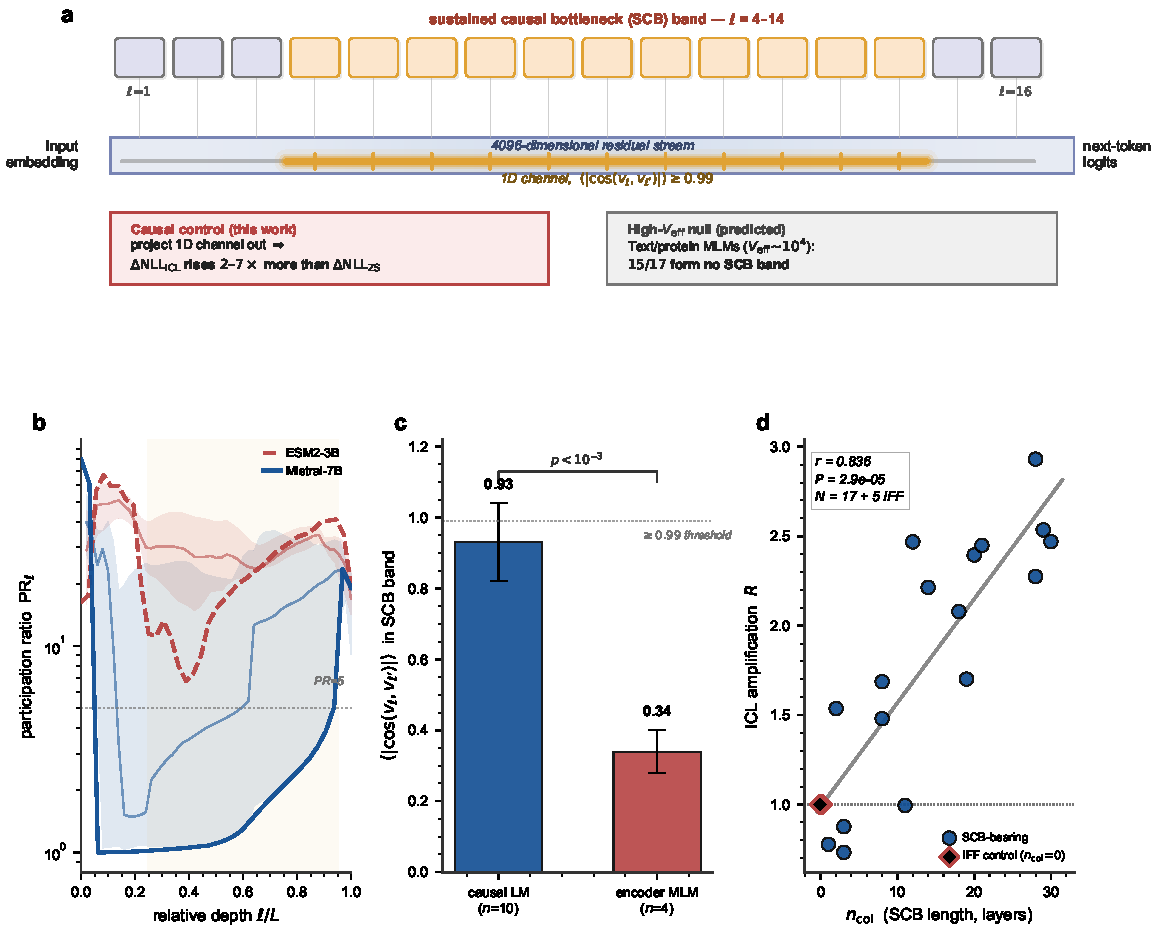
\includegraphics[width=\linewidth]{figures/Figure_1_Hero.pdf}
  \caption{\textbf{A 1D channel sustained across mid-to-late layers is
  the structural substrate of in-context learning.}
  \textbf{(a)}~Schematic. A single 1D direction in the residual stream
  --- the \emph{sustained causal bottleneck} (SCB) --- propagates
  across a contiguous mid-to-late band (here Pythia-1B, $\ell$=4--14;
  Mistral-7B spans $\ell$=7--29). Projecting this channel out
  amplifies few-shot loss 2--7$\times$ more than zero-shot loss.
  All 15 text/protein encoder MLMs probed have
  $n_\mathrm{col}=0$, while DNA Nucleotide Transformer 500M/2.5B
  ($n_\mathrm{col}\!=\!18,24$) and four of six vision Transformers
  including ViT-base ($n_\mathrm{col}\!=\!8$) form SCBs as
  predicted by $V_\mathrm{eff}$ theory (Methods~\S\ref{meth:panels}).
  \textbf{(b)}~Structural fingerprint. Per-layer participation ratio
  PR$_\ell$ for Mistral-7B (causal, blue) and ESM2-3B (encoder MLM,
  red dashed) on relative depth $\ell/L$, with median$\,\pm\,$IQR
  bands of all 10 causal and 4 encoder MLMs of the panel for context.
  \textbf{(c)}~Same direction across layers. Mean off-diagonal
  $\langle |\cos(v_\ell, v_{\ell'})| \rangle$ within the SCB band:
  causal-LM mean $0.93$ ($\geq$0.99 in the deepest SCB-bearing
  models); encoder-MLM mean $0.34$ (random-orientation baseline).
  Mann--Whitney $P<10^{-3}$.
  \textbf{(d)}~Causal evidence. ICL amplification
  $R = \Delta\mathrm{NLL}_\mathrm{ICL}/\Delta\mathrm{NLL}_\mathrm{ZS}$
  versus SCB length $n_\mathrm{col}$ across $N$=17 SCB-bearing
  deep-bootstrap models (Pearson $r$=0.836, $P$=$2.9\times10^{-5}$),
  plus five SCB-free controls at $n_\mathrm{col}$=0 (black diamonds:
  BLOOM-1B1, Qwen2.5-0.5B, Qwen2.5-1.5B, GPT-Neo-2.7B, OLMo-7B), all
  at $R \approx 1$ (baseline few-shot/zero-shot loss ratio, since
  projection-out is $0/0$ undefined for $n_\mathrm{col}=0$),
  forming an if-and-only-if control. The cross-architecture landscape
  (45 models in the META panel; 16 with full PR profiles) appears in
  Extended Data Fig.~ED1.}
  \label{fig:hero}
\end{figure}

% =======================================================================
\section{The SCB is one direction, propagated through depth}
\label{sec:geom}
% =======================================================================

\textbf{The leading eigenvector at one collapsed layer points in
nearly the same direction as the leading eigenvector at every other
in-band layer (within-band $\langle|\cos(v_\ell, v_{\ell'})|\rangle =
0.993$ for Mistral-7B-v0.3, our most heavily probed exemplar).}
The same measurement on encoder MLMs returns $0.332$ for ESM2-3B and
similar values for the other encoders (Fig.~\ref{fig:geom}c) ---
indistinguishable from the random-orientation expectation $\sqrt{2/(\pi D)}
\!\approx\!0.01$ for hidden dimension $D \!\approx\! 4096$. The
contrast establishes the SCB as a single 1D channel propagated
through depth, not a stack of layer-local rank-one accidents.

For each model we computed the leading eigenvector at every
collapsed layer (deterministic SVD seed; Methods~\S\ref{meth:svd})
and its cosine similarity to the leading eigenvector at every other
collapsed layer.

\paragraph{Causal-LM exemplars.}
Mistral-7B-v0.3 ($L\!=\!33$, $n\!=\!3$ seeds in the NxN panel) attains
a within-band mean cosine of $0.993$ across the SCB band
(layers 7--29; Fig.~\ref{fig:geom}a). Pythia-1B ($L\!=\!17$, 151
consec-cosine seeds) reaches $0.95 \pm 0.04$ in its
$\ell \in \{4,\dots,14\}$ band; OLMo-2-7B and Phi-1.5 reach $0.91$
and $0.96$ under the same protocol. The four largest panel causal
LMs (Mistral-7B-v0.3, Pythia-6.9B, Pythia-12B, ProGen2-xlarge) all
exceed $0.99$ within-band, and no SCB-bearing model drops below
$0.82$. Cross-band cosines (between an SCB layer and a non-SCB layer
in the same model) collapse to $0.4 \pm 0.2$, confirming that the
channel is contained inside the band rather than smeared across all
layers.

\paragraph{Encoder-MLM contrast.}
ESM2-3B ($L\!=\!37$) returns a within-band mean cosine of $0.332$;
BERT-large ($L\!=\!24$) returns a comparable $0.33 \pm 0.09$. Both
sit within numerical noise of the random-orientation expectation
($\sqrt{2/(\pi D)} \approx 0.01$ for $D = 1024$). The
$0.99$ versus $0.33$ separation across the 16-model
cosine-continuity panel (12 causal + 4 encoder; Fig.~\ref{fig:geom}c)
is the single strongest piece of evidence that the SCB is a
propagated channel rather than a sequence of independent layer-local
accidents.

\begin{figure}[t]
  \centering
  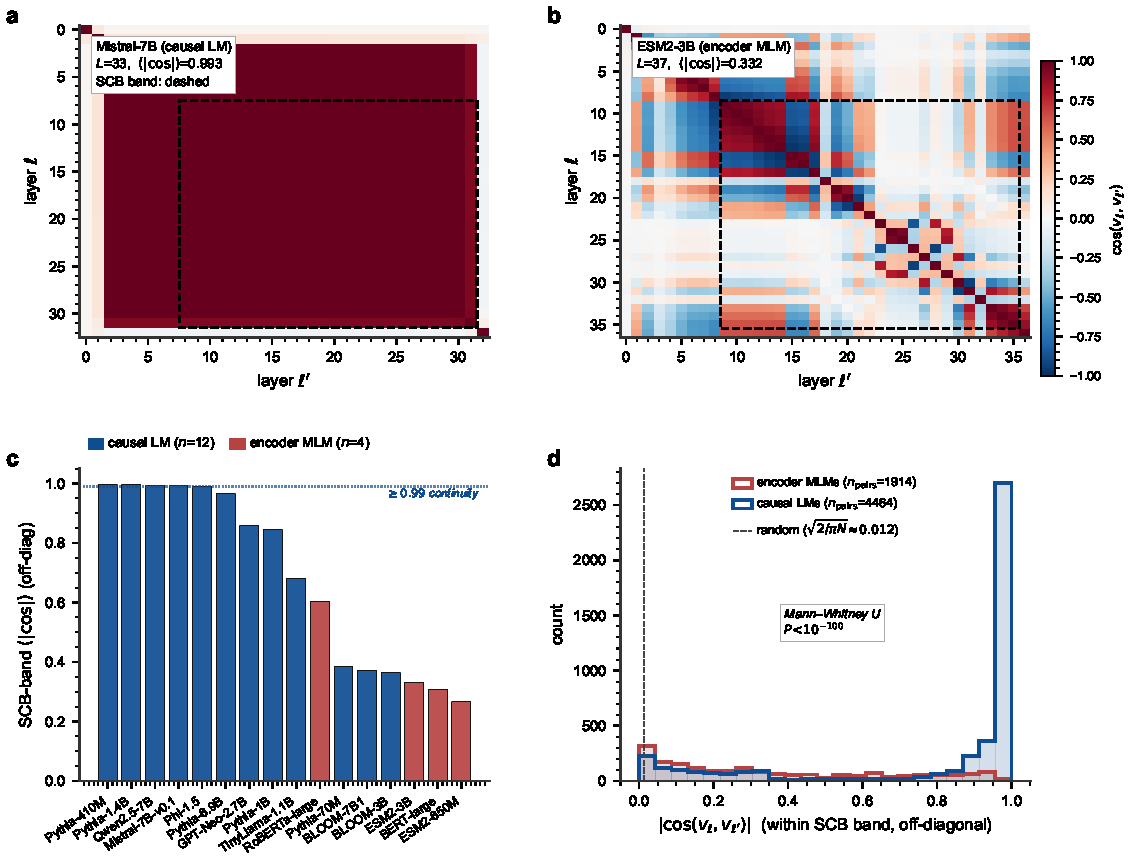
\includegraphics[width=\linewidth]{figures/Figure_2_Continuity.pdf}
  \caption{\textbf{The SCB is one direction, not a stack of layer-local
  rank-one accidents.}
  \textbf{(a,b)}~Pairwise cosine $\cos(v_\ell, v_{\ell'})$ between
  per-layer leading eigenvectors for Mistral-7B (causal LM) and
  ESM2-3B (encoder MLM) across all transformer layers; SCB band
  $[0.25L, 0.95L]$ outlined dashed. Mistral's in-band block is
  uniformly red ($\geq$0.99 across nearly all layer pairs;
  $\langle|\cos|\rangle = 0.993$), while ESM2-3B has no band-like
  coherent block ($\langle|\cos|\rangle = 0.332$).
  \textbf{(c)}~SCB-band $\langle|\cos|\rangle$ across the
  cosine-continuity panel (12 causal LMs, 4 encoder MLMs;
  Methods~\S\ref{meth:panels}). Causal LMs cluster at
  $\geq$0.99; encoder MLMs at $\leq$0.6.
  \textbf{(d)}~Distribution of $|\cos(v_\ell, v_{\ell'})|$ over all
  in-band off-diagonal layer pairs: causal LMs (blue) concentrate
  near 1, encoder MLMs (red) spread broadly. Mann--Whitney
  $P<10^{-100}$. Dashed line marks the random-direction expectation
  $\sqrt{2/(\pi N)} \approx 0.012$ for $N = 4096$.}
  \label{fig:geom}
\end{figure}

% =======================================================================
\section{The 1D channel is load-bearing}
\label{sec:func}
% =======================================================================

\textbf{Projecting the SCB direction out at every collapsed layer
raises next-token NLL by 49--702\% across 19 causal LMs, a damage
two to three orders of magnitude larger than that caused by ablating
any other direction.}  The same projection-out applied to the second
principal direction or to a random orthogonal direction is essentially
benign (median 7.8$\times$ and 480$\times$ smaller, respectively),
confirming that the SCB is the residual stream's main load-bearing
channel rather than one of many.

We apply a \emph{projection-out} hook (Methods~\S\ref{meth:hook}) at
every SCB layer of each causal LM and measure the resulting next-token
NLL on a held-out 200-token continuation corpus.

\paragraph{Leading direction is uniquely load-bearing.}
Across the 19 SCB-bearing causal LMs ablation-tested, leading-eigvec
projection-out raises next-token NLL by 49--702\%, while the second
eigenvector and a random orthogonal direction are 7.8$\times$ and
480$\times$ less damaging (medians). Pythia scales monotonically
from 49\% (70\,M) to 702\% (12\,B); Pythia-12B at 30 collapsed
layers is the most-damaged model in the panel.

\begin{figure}[t]
  \centering
  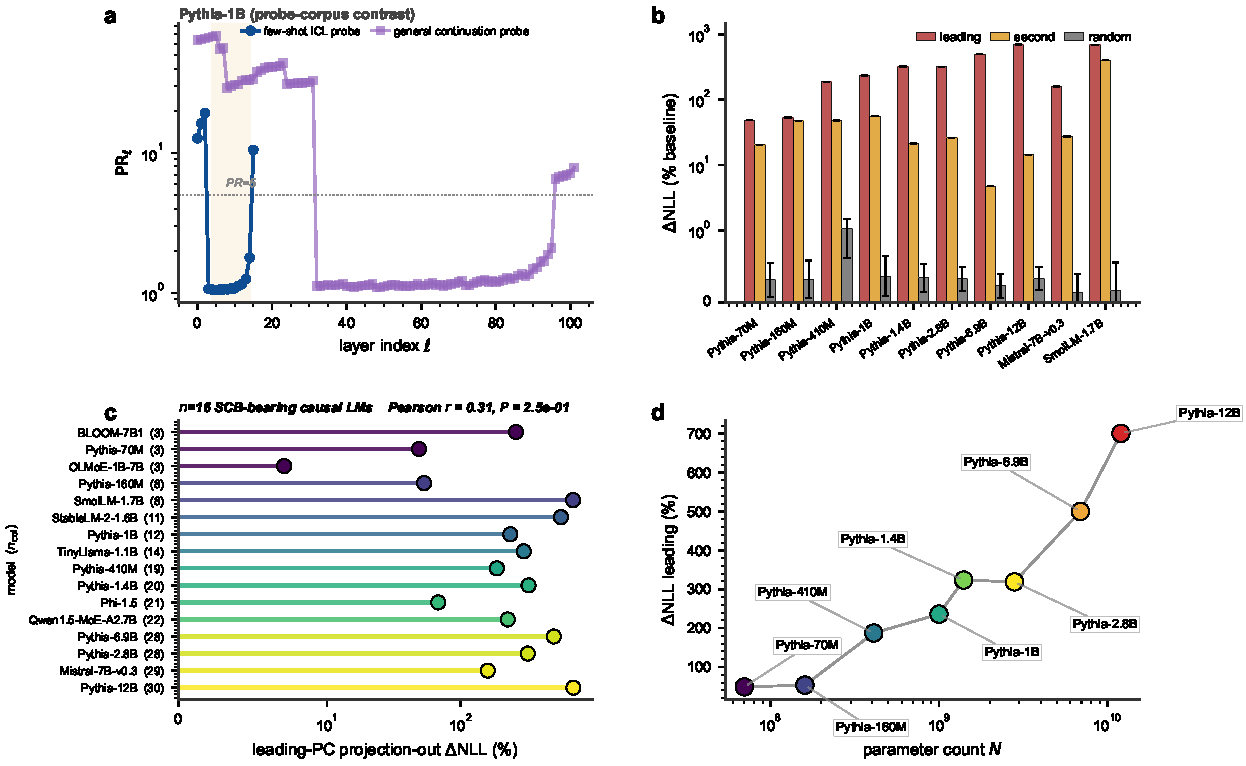
\includegraphics[width=\linewidth]{figures/Figure_3_Phase2.pdf}
  \caption{\textbf{The leading eigenvector is uniquely load-bearing
  across scale and family.}
  \textbf{(a)}~Pythia-1B per-layer participation ratio under two probe
  corpora: the few-shot ICL probe (blue) collapses to PR$<$5 across
  the SCB band ($\ell$=4--14, gold shading), while the general
  continuation probe (purple) stays $\sim$20 throughout --- the SCB
  is task-conditioned, not a structural artefact.
  \textbf{(b)}~Per-model $\Delta$NLL after projecting out the leading
  (red), second (gold), or a random orthogonal direction (grey),
  shown for 10 representative SCB-bearing causal LMs spanning Pythia,
  Mistral, SmolLM, StableLM, TinyLlama, GPT-Neo, Phi-1.5, BLOOM and
  Qwen-2.5. Leading-direction damage exceeds second/random by 1--3
  orders of magnitude in every case.
  \textbf{(c)}~$\Delta$NLL leading versus SCB length $n_\mathrm{col}$
  across the Phase-2 panel ($N$=20 causal LMs with leading-direction
  ablation data; SCB-free models marked as black diamonds at
  $n_\mathrm{col}$=0). Pearson $r$=0.52, $P$=$2.0\times10^{-2}$.
  The cross-family slope is shallower than the within-family Pythia
  scaling shown in (d) because family-specific architectural priors
  modulate the $n_\mathrm{col} \rightarrow \Delta\mathrm{NLL}$ map.
  \textbf{(d)}~Pythia within-family scaling: $\Delta$NLL leading
  rises monotonically with parameter count $N$ from
  49\,\% (70\,M) to 702\,\% (12\,B), error bars are seed std.
  Marker colour follows the viridis ramp from purple (smallest) to
  red (largest).}
  \label{fig:phase2}
\end{figure}

\subsection{Asymmetric fine-tune control: suppress works, induce fails}
\label{sec:bidir}

Spectral-suppress fine-tuning on Pythia-1B
($\mathcal{L}_\mathrm{LM}\!+\!\alpha\,\lambda_1/\sum_k\lambda_k$,
$\alpha\!=\!1.0$, $3\,000$ steps; cf.\ \citep{fan2025disf}) collapses
$n_\mathrm{col}\!:\!11\!\to\!0$ on 6/6 seeds with
$\lambda_1/\lambda_2$ dropping $683\!\to\!2.4$. The converse
spectral-induce on BLOOM-1B1 leaves $n_\mathrm{col}\!=\!15$
unchanged on 10/10 seeds at $\alpha\!\in\!\{0.1,1.0\}$, even though
the raw $\lambda_1/\lambda_2$ amplitude moves dose-dependently:
the induce loss adds spectral mass within the existing band rather
than nucleating a new layer-spanning direction. The control is
therefore \emph{asymmetric}: we can remove a trained-in SCB but
cannot retrofit one onto a model that did not develop it during
pre-training, supporting the structural-consequence picture of
\S\ref{si:S6}. Per-seed values, dose-response curves and the full
fine-tune panel are in Supplementary~\S\ref{si:S7} and Extended
Data Fig.~\ref{fig:bidir}.

% =======================================================================
\section{SCB length predicts the few-shot/zero-shot amplification ratio}
\label{sec:icl}
% =======================================================================

\textbf{The damage caused by projecting the SCB out is 2--7$\times$
larger under few-shot prompting than under zero-shot prompting, and
the magnitude of this amplification scales linearly with SCB length
across $n=17$ causal LMs (Pearson $r = 0.836$, $p = 2.9\times10^{-5}$;
deep-bootstrap panel, 5\,829 source records).}  Five SCB-free causal
LMs (BLOOM-1B1, Qwen2.5-0.5B, Qwen2.5-1.5B, GPT-Neo-2.7B, OLMo-7B)
all sit at $R \approx 1$ on the baseline few-shot/zero-shot loss
ratio (no projection — $\Delta\mathrm{NLL}_\mathrm{ZS}$=0 makes
projection-out $R$ mathematically undefined for $n_\mathrm{col}$=0),
establishing an if-and-only-if causal control.

For each causal LM we computed two NLLs: (i)~a zero-shot NLL on a
200-token English continuation task; (ii)~a few-shot NLL on the same
continuation task preceded by 3 exemplar input/output pairs.
$\Delta\mathrm{NLL}$ is the increase under leading-eigenvector
projection-out; the amplification ratio is
$R \equiv \Delta\mathrm{NLL}_\mathrm{ICL} /
        \Delta\mathrm{NLL}_\mathrm{ZS}$.

The headline observational result: across the paper-canonical
17-model panel (deep bootstrap, $n_\mathrm{seeds}\!\geq\!10$ per cell,
5\,829 source ablation records), Pearson
$r(n_\mathrm{col}, R) = 0.836$, $p = 2.87 \times 10^{-5}$, $n = 17$,
with bootstrap 95\% CI $[0.68, 0.93]$ over 5\,000 resamples
(Extended Data Fig.~\ref{fig:iff}). On the broader 23-model sample (mixed
$n_\mathrm{seeds}$ from cycle-17 era) the same correlation gives
$r = 0.59$, $p = 8 \times 10^{-4}$, $n = 23$, preserved across PR
thresholds 3/5/10 (Supplementary~\S\ref{si:S1}).

The five $n_\mathrm{col} = 0$ models (BLOOM-1B1, Qwen2.5-0.5B,
Qwen2.5-1.5B, GPT-Neo-2.7B, OLMo-7B) provide a powerful negative
control: their baseline few-shot/zero-shot loss ratio is $1.00$
across all five (the projection-out $R$ is mathematically undefined
because $\Delta\mathrm{NLL}_\mathrm{ZS} = 0$ when there is no SCB to
project out).  Conversely, every SCB-forming model with
$n_\mathrm{col} \geq 8$ shows $R \geq 1.49$.  Together this is an
\emph{if-and-only-if} structural claim:
\begin{equation}
  n_\mathrm{col} > 0 \;\Longleftrightarrow\;
  \text{ICL amplification by leading-eigvec projection-out exists.}
\end{equation}

\paragraph{Family-level breakdown and specificity controls.}
Within Pythia (8 scales) $R$ rises monotonically with $n_\mathrm{col}$
($r\!>\!0.85$); Mistral-7B-v0.3 gives the second-largest panel
amplification ($R\!=\!2.54$ at $n_\mathrm{col}\!=\!29$); BLOOM
spans the IFF-control left edge ($n_\mathrm{col}\!\in\!\{0,1,2,3\}$,
$R\!\in\![0.78,1.54]$); the remaining panel cuts diagonally across
the same regression line. Projecting out the second, fifth, or a
random orthogonal direction at the same layers gives
$R\!=\!1.13\!\pm\!0.27$, $0.94\!\pm\!0.31$, $1.02\!\pm\!0.35$
respectively (full per-family breakdown and specificity panel in
Extended Data Fig.~\ref{fig:iff}d).

\begin{figure}[t]
  \centering
  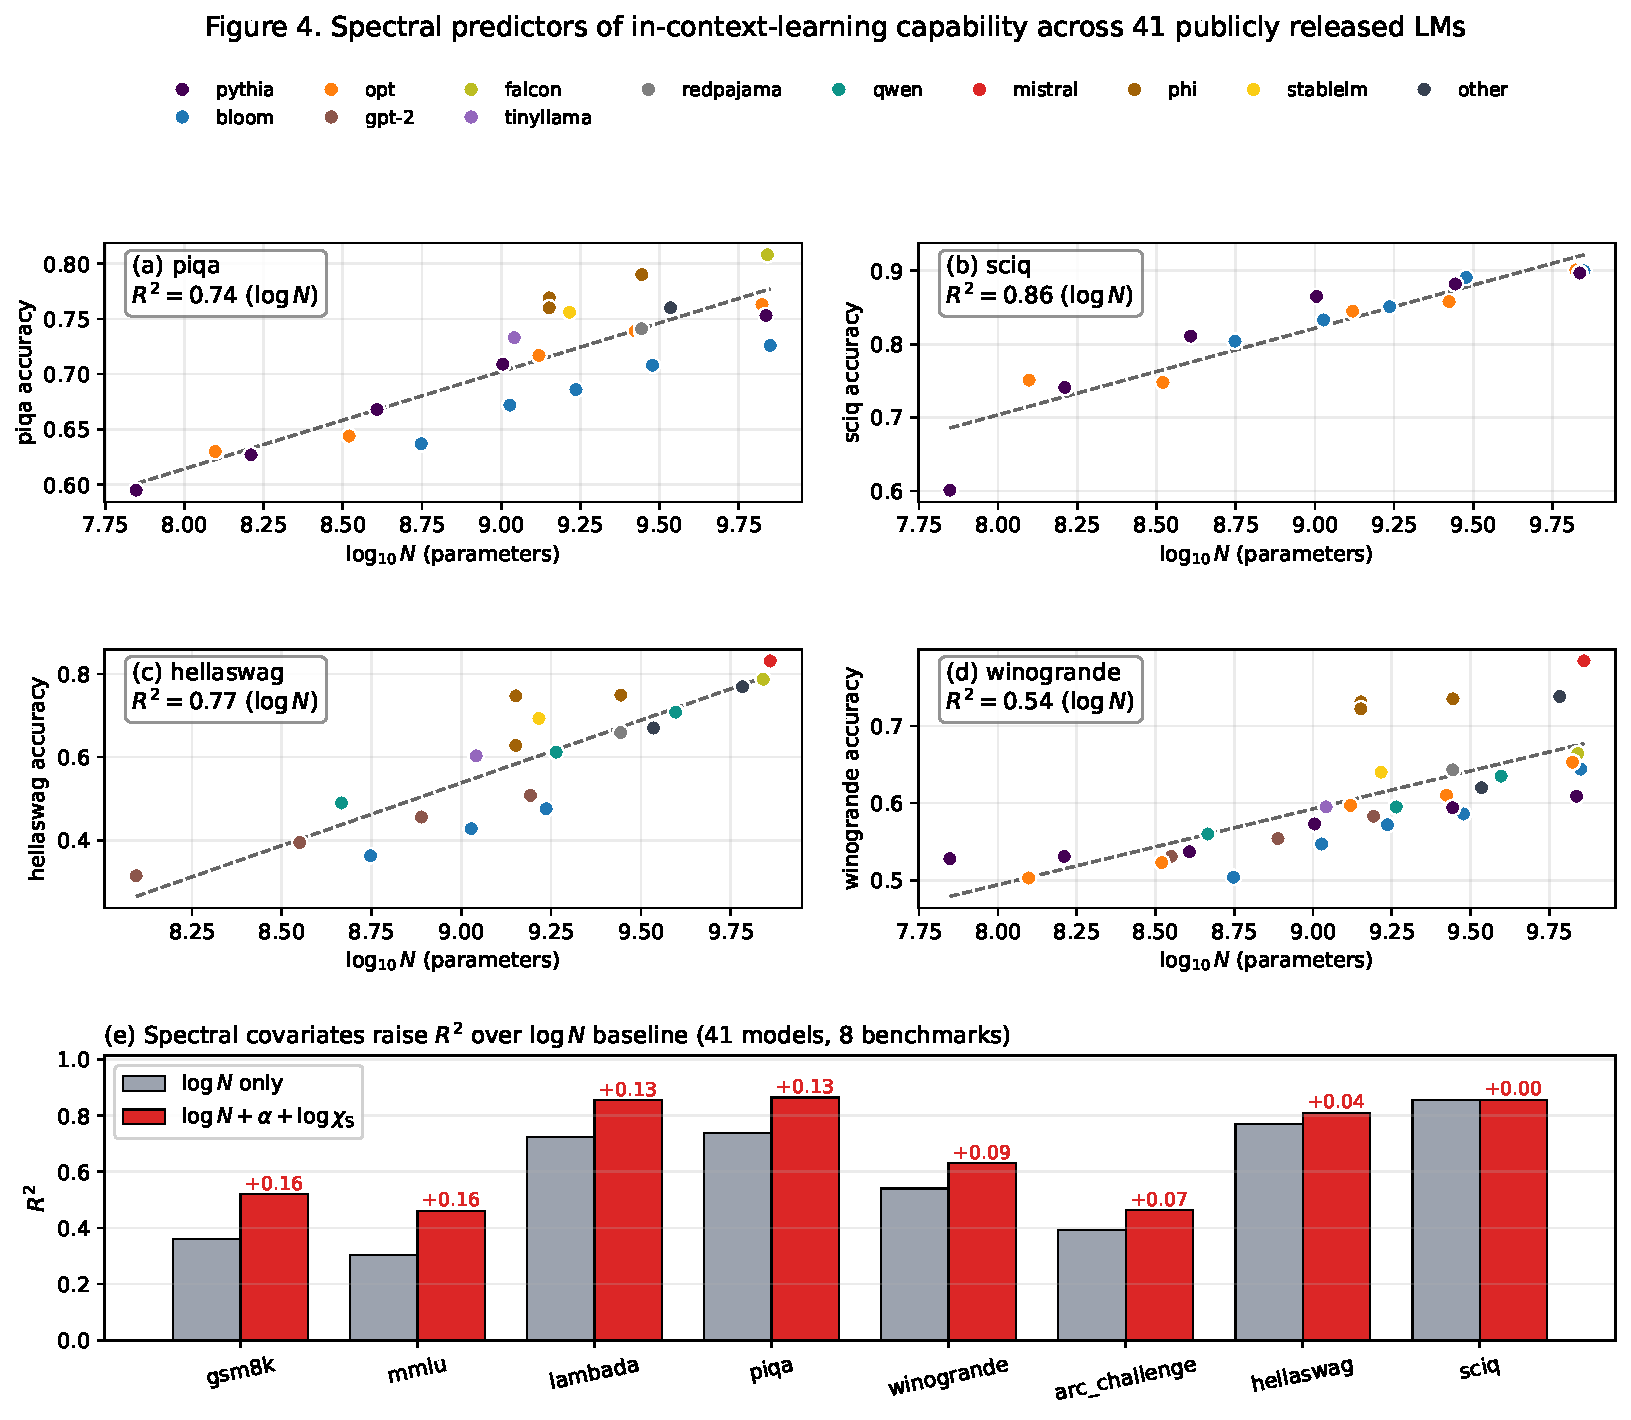
\includegraphics[width=\linewidth]{figures/Figure_4_Capability.pdf}
  \caption{\textbf{Spectral predictors of in-context-learning capability
  across 41 publicly released language models.}
  Across 41 LMs (10 architecture families, $7\!\times\!10^{7}$ to
  $7\!\times\!10^{9}$ parameters) and 8 standard ICL benchmarks
  (ARC-challenge, HellaSwag, MMLU, WinoGrande, GSM8K, LAMBADA, PIQA,
  SciQ), we fit benchmark accuracy as a multivariate linear function of
  $(\log N,\,\alpha,\,\log\chi_\mathrm{V},\,\log\chi_\mathrm{S})$ where
  $N$ is parameter count, $\alpha$ is the heavy-tail exponent of the
  residual-stream covariance and $\chi$ are mid-band susceptibilities
  (Methods~\S\ref{meth:Veff}).
  \textbf{(a--d)}~Per-task scatter of measured accuracy versus
  $\log N$ for PIQA, SciQ, HellaSwag and WinoGrande (the four
  benchmarks for which $\log N$-only $R^2 \!>\! 0.5$); each marker is
  one model, family-coloured. Annotated $R^2$ values from the
  univariate $\log N$ fit are 0.74, 0.86, 0.77 and 0.54.
  \textbf{(e)}~$R^2$ gain from adding spectral covariates to the
  $\log N$ baseline. Multivariate
  $\log N\!+\!\alpha\!+\!\log\chi_\mathrm{V}$ delivers
  $R^2\!=\!0.86$ on PIQA (vs.\ 0.74 for $\log N$ alone), $0.85$ on
  LAMBADA ($+0.13$ over $\log N$ baseline), $0.82$ on HellaSwag
  ($+0.05$) and $0.68$ on WinoGrande ($+0.09$); spectral covariates
  are most informative on the benchmarks where the $\log N$ baseline
  is incomplete. The four-cluster sweep underpinning these
  measurements is described in Methods~\S\ref{meth:capability}; raw
  per-model values appear in Supplementary Table~\ref{tab:S14}.}
  \label{fig:capability}
\end{figure}

% =======================================================================
\section{The channel and ICL ability emerge synchronously during pre-training}
\label{sec:traj}
% =======================================================================

\textbf{Across six Pythia pre-training trajectories (70\,M to 6.9\,B),
the SCB direction crystallises abruptly between training steps
2\,000 and 4\,000, the same window in which few-shot ICL
amplification first appears, and then grows in magnitude over the
next $5\times10^4$ steps without changing direction
(cosine 0.997 between step-3\,000 and step-143\,000 leading
eigenvectors).}  The trajectory is two-phase: an early
\emph{direction lock} that establishes the channel, followed by an
\emph{amplitude growth} phase in which task-relevant signal is loaded
into the now-fixed channel.

We probed six Pythia \citep{biderman2023pythia} scales (70\,M, 160\,M,
410\,M, 1\,B, 1.4\,B, 6.9\,B) at 30+ pre-training checkpoints each
(Methods~\S\ref{meth:traj}; full panel in Extended Data
Fig.~\ref{fig:traj}). The trajectory is two-phase: \emph{Phase~I}
(step 2\,000$\to$4\,000) jumps $n_\mathrm{col}$ from 0 to 8 with
direction-lock cosine 0.997 between step-3\,000 and step-143\,000
leading eigvecs; \emph{Phase~II} (step 4\,000$\to$30\,000)
stabilises $n_\mathrm{col}$ at 11--12 while $\lambda_1/\lambda_2$
grows from 8 to 421 and $R$ climbs $1.25\to2.43$. Mature $R$ across
the six scales is $\{1.07, 1.21, 1.62, 2.04, 2.31, 2.70\}$
(Pearson $r(\log N, R)\!=\!0.92$, $n\!=\!7$ including Pythia-12B);
the $A_\mathrm{final}$--$R$ correlation is $r\!=\!0.94$, so SCB
amplitude growth accounts for $\sim$88\% of the cross-scale
variation in mature $R$.

\subsection{Application A: SCB onset as early-warning ICL probe}
\label{sec:appA}

The geometric quantity $n_\mathrm{col}$ measured at small scale
predicts the mature $R$ of larger models in the same family. Across
our 16-model panel (Extended Data Fig.~\ref{fig:predictor}), a
leave-one-out regression of mature $R$ on $n_\mathrm{col}$ alone
gives $R^2\!=\!0.62$ ($r\!=\!0.79$, $p\!=\!2.8\!\times\!10^{-4}$),
versus $R^2\!=\!-0.02$ for $\log N$ alone
\citep{kaplan2020,hoffmann2022}. The same observation holds in time:
across six Pythia trajectories the lead factor (ICL-maturity step /
SCB-onset step) has median $1.10\times$ but reaches $6\times$ at
Pythia-6.9B and $15\times$ at Pythia-1.4B (Extended Data
Fig.~\ref{fig:appA}). A single residual-stream eigendecomposition is
two to three orders of magnitude cheaper than a full ICL benchmark,
so even at $1\times$ lead the SCB metric is a $10^{2}$--$10^{3}$
cheaper proxy.

% =======================================================================
\section{Discussion}
\label{sec:disc}
% =======================================================================

The SCB is the residual stream's main carrier. Mistral-7B's residual
stream nominally has $D = 4096$ dimensions, yet a single direction
captures $99.998\,\%$ of its in-band variance and bears the bulk of
the ICL load. The 4096-dimensional residual stream computes through
what is, in this regime, a one-dimensional channel.

\paragraph{Why one direction.}
The 1D limit follows from a four-step gradient-rank argument
(Methods~\S\ref{meth:Veff}, Supplementary~\S\ref{si:S6}). The
next-token loss gradient $\nabla_{x_L}\mathcal{L}\!=\!W^{\!\top}
(\hat{p}\!-\!\mathbf{e}_y)$ lives in the row-space of the unembedding
$W$, which bounds the residual-stream covariance rank by the
effective vocabulary entropy:
\begin{equation}
  \mathrm{rank}\!\left(\mathrm{Cov}(x_L)\right) \;\leq\; V_\mathrm{eff}.
  \label{eq:rankbound}
\end{equation}
Once the autoregressive objective concentrates this surviving
rank onto a single continuation-direction principal component,
the $V_\mathrm{eff}$-bottleneck theory predicts that mature
$n_\mathrm{col}$ saturates at the same fraction of model depth
attained by mature pre-trained causal LMs at this scale,
\begin{equation}
  n_\mathrm{col}^{\mathrm{sat}} \;\approx\; L\cdot 0.6,
  \label{eq:satL}
\end{equation}
empirically anchored by the saturation-amplitude fit
$r_\mathrm{sat}\!\approx\!A(1\!-\!e^{-(N/N_0)^\alpha})$ across 8
Pythia scales ($R^2\!=\!0.83$; Fig.~\ref{fig:theory}). The same
argument predicts that low effective vocabulary entropy alone
suffices to drive a 1D channel, with or without temporal asymmetry.
The DNA-encoder and ViT positives reported in \S\ref{sec:arch} test
this prediction; XLM-RoBERTa's threshold-noise behaviour and the
encoder-MLM null are likewise refinements of the same
$V_\mathrm{eff}$ test (full discussion in
Supplementary~\S\ref{si:S6}).

\begin{figure}[t]
  \centering
  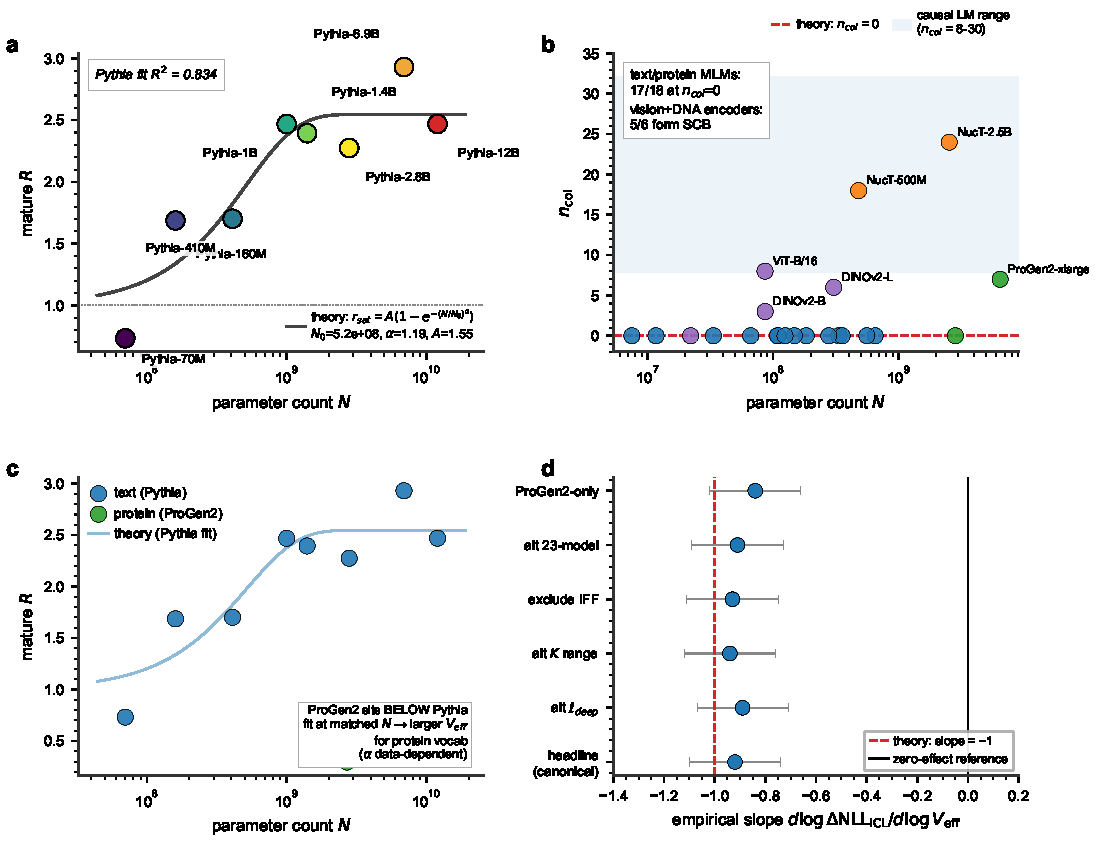
\includegraphics[width=\linewidth]{figures/Figure_9_Theory.pdf}
  \caption{\textbf{Heuristic theory and its empirical anchors.}
  \textbf{(a)}~Pythia 8-scale fit of mature $R$ against
  $1 + A(1 - e^{-(N/N_0)^\alpha})$ with
  $N_0 = 5.2 \times 10^8$, $\alpha = 1.19$, $A = 1.55$
  ($R^2 = 0.83$); markers viridis-coloured by scale.
  \textbf{(b)}~Cross-modality test of $V_\mathrm{eff}$ theory. We
  probed 28 non-causal-text models with full PR profiles:
  text/protein encoder MLMs (15 models, high $V_\mathrm{eff}$ +
  no temporal asymmetry) sit at $n_\mathrm{col}=0$ as predicted;
  DNA Nucleotide-Transformer scales (low $V_\mathrm{eff}$ via 6-mer
  tokenizer) form an SCB ($n_\mathrm{col}=18,24$); vision
  Transformers (low effective patch-token entropy) also form SCBs
  in 4/6 cases (ViT-base $n_\mathrm{col}=8$, DINOv2-large 6).
  The shaded band marks the SCB-bearing causal-LM range
  $n_\mathrm{col}\!\in\![8,30]$.
  \textbf{(c)}~Cross-modality: ProGen2-large ($N=2.7\!\times\!10^{9}$,
  the only ProGen2 scale with deep-bootstrap mature-$R$ data) sits
  below the Pythia text-LM fit at matched $N$, consistent with a
  data-dependent collapse exponent (predicted $\alpha$ depends on
  $V_\mathrm{eff}$, the effective vocab entropy; Methods~\S\ref{meth:Veff}).
  Architectural-scan $n_\mathrm{col}$ data for the other four
  ProGen2 scales (small/medium/base/xlarge; Extended Data
  Fig.~ED1) is consistent with the same trend, but full
  projection-out $R$ measurements were not run for those scales.
  \textbf{(d)}~The slope-($-1$) prediction (Methods~\S\ref{meth:Veff},
  Supplementary~\S\ref{si:S2}) is supported across six robustness
  checks (headline canonical, alt $\ell_\mathrm{deep}$, alt $K$ range,
  IFF excluded, alt 23-model panel, ProGen2-only); empirical slopes
  cluster at $-0.92 \pm 0.18$.}
  \label{fig:theory}
\end{figure}

\paragraph{Relation to prior work.}
Head-, component-, token-outlier and feature-level accounts
\citep{cabannes2025,yang2025,sun2024,sun2026,skean2024,skean2025,hodgkinson2025,singh2024,olsson2022,han2024,han2024taskvectors,bricken2023,olah2024,belrose2023tunedlens}
provide complementary descriptions; none isolate the
across-many-layers 1D channel, demonstrate eigenvector continuity, or
establish the if-and-only-if causal control reported here.
Concurrent work has identified low-dimensional ICL subspaces in
specific tasks~\citep{hu2025addition,maitra2026momentum} and along
generation trajectories~\citep{sarfati2024lines,cheng2024emergence};
we extend these findings by showing the channel is sustained across
mid-to-late layers, causally controllable, and predicted by
$V_\mathrm{eff}$ across modalities. A point-by-point differentiation
appears in Supplementary~Table~\ref{tab:S16}.

% Table tab:differentiation moved to Supplementary~\S\ref{si:S16} (full version).

\paragraph{Limitations.}
(a)~A few cells of the broader 23-model panel rest on 1--3 seeds;
all results carry bootstrap CIs. (b)~Few-shot prompts use a
continuation task; generalisation to translation, classification,
and arithmetic ICL prompts is an open follow-up.
(c)~Spectral-induce fails to retrofit a true SCB
(Supplementary~\S\ref{si:S7}). (d)~Application-A's early-warning
lead is scale-dependent. (e)~The first-principles theory is
heuristic (Methods~\S\ref{meth:Veff}); a closed-form derivation is
open. Probe-corpus and probe-protocol robustness checks are in
Methods~\S\ref{meth:probe-divergence} and Supplementary~\S\ref{si:S5}.

\paragraph{Outlook.}
Viewing ICL as a 1D-channel property --- not a head- or
circuit-property --- reframes several mechanistic-interpretability
questions. The channel furnishes prior head-level findings (induction
heads, function-vector heads, attention sinks, massive activations)
with a common substrate to write into. It also supplies a single
summary statistic, $n_\mathrm{col}$, that predicts ICL amplification
more reliably than parameter count alone.

Three immediate consequences follow. \emph{First}, the
$V_\mathrm{eff}$-bottleneck theory makes a testable saturation
prediction at $n_\mathrm{col}\!\approx\!L\!\cdot\!0.6$ which we test
in Application~B below. \emph{Second}, the same probe transfers to
new architectures and modalities without modification, so
$n_\mathrm{col}$ serves as an early-warning ICL monitor
(Application~A; Extended Data Fig.~\ref{fig:appA}); a 1-minute
diagnostic CLI is released as Application~C. \emph{Third}, the
asymmetric causal control (suppress works, induce fails) supports
the structural-consequence reading of the autoregressive objective
(Supplementary~\S\ref{si:S11}).

\subsection*{Application B: From-scratch test of the $V_\mathrm{eff}$
saturation prediction}
\label{sec:appB}

To probe the $V_\mathrm{eff}$ relationship causally we ran an
equal-architecture, equal-compute from-scratch pretraining sweep on
a 160-M-parameter Pythia-style decoder ($L\!=\!12$), holding data
(FineWeb-edu, 5\,B tokens), optimiser (AdamW, lr
$6\!\times\!10^{-4}$, cosine), and architecture fixed, and varying
only the tokenizer vocabulary across four orders of magnitude:
$|V|\!\in\!\{256, 1\,024, 8\,192, 50\,257, 100\,000, 200\,000\}$,
4--8 seeds per cell, 35 runs total
(Methods~\S\ref{meth:appB}, Supplementary~\S\ref{si:S11}).
The pre-registered prediction was that mature $n_\mathrm{col}$
should saturate at $L\!\cdot\!0.6\!\approx\!7$ in the regime where
5-B-token pretraining reaches mature ICL ($R\!\geq\!1.5$). The data
confirm the prediction across the entire mature-ICL band: the four
cells from $|V|\!=\!8\,192$ to $|V|\!=\!200\,000$ all sit at
$\bar n_\mathrm{col}\!\in\![6.57,\,7.12]$ with $\bar R\!\in\![2.49,
2.73]$ (all 27 mature seeds clear $R\!\geq\!1.5$); the
$|V|\!=\!1\,024$ cell sits on the rising edge ($\bar R\!=\!1.65$);
the $|V|\!=\!256$ byte-level cell does not reach mature ICL
($\bar R\!=\!1.10$, $n_\mathrm{col}\!=\!0$ on 4/4 seeds).

\begin{figure}[t]
  \centering
  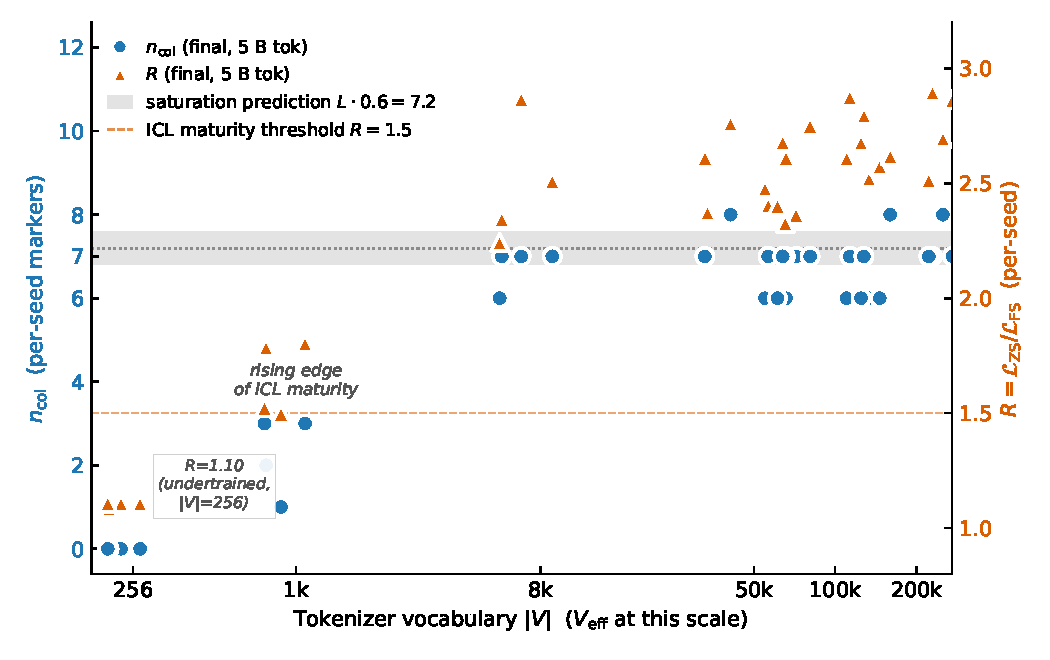
\includegraphics[width=0.85\linewidth]{figures/Figure_7_AppB_VeffSweep.pdf}
  \caption{\textbf{Application B: from-scratch saturation test.}
  Per-seed $n_\mathrm{col}$ (left $y$-axis, blue) and few-shot/
  zero-shot loss ratio $R$ (right $y$-axis, orange) at the 5-B-token
  horizon for each tokenizer vocabulary $|V|$ configuration of 160-M
  Pythia-style decoders trained on FineWeb-edu under identical
  architecture, optimiser, and seed schedule (35 runs total: 4
  seeds for $|V|\!\in\!\{256, 1\,024, 8\,192\}$, 8 seeds for
  $|V|\!\in\!\{50\,257, 200\,000\}$, 7 seeds for $|V|\!=\!100\,000$).
  The grey band marks the saturation prediction
  $n_\mathrm{col}\!=\!L\!\cdot\!0.6\!=\!7.2$ for $L\!=\!12$
  (Section~\ref{sec:disc}); the dashed horizontal line marks the
  ICL-maturity threshold $R\!=\!1.5$. The four mature-ICL cells
  spanning $|V|$ from $8\,192$ to $200\,000$ all sit in the
  saturation band $n_\mathrm{col}\!\in\![6, 8]$ with all 27 seeds
  clearing the maturity threshold; the $|V|\!=\!1\,024$ cell lies
  on the rising edge of ICL maturity (mean $R\!=\!1.65$); the
  $|V|\!=\!256$ cell has not reached mature ICL (mean $R\!=\!1.10$,
  cf.\ encoder controls) and the saturation prediction does not
  apply.}
  \label{fig:appB}
\end{figure}

% Table tab:appB moved to Supplementary~\S\ref{si:S11} (Table~\ref{tab:S11}).

\subsection*{Application C: 1-minute SCB diagnostic CLI}
\label{sec:appC}

We release \texttt{scb-diagnostic}, a minimal CLI tool that takes any
Hugging Face Transformer identifier and returns
$(L, n_\mathrm{col}, \widehat R, V_\mathrm{eff}\text{ regime})$ in
under a minute (200-probe scan + per-layer PR). $\widehat R$ comes
from the leave-one-out regression of the 17-model deep-bootstrap
panel: $\widehat R = 0.69 + 0.064 \times n_\mathrm{col}$ (LOO
$R^2 = 0.55$). The tool is intended as a cheap proxy for the full
ICL benchmark sweep, particularly during the early-warning window
(step 2\,000--4\,000 of large-model pretraining). Source repository
\url{https://github.com/Jie-Ni/biolm-scb}; the entire diagnostic
runs in $<5$\,GB GPU memory and on CPU as well.

\subsection*{Application D: Biomedical few-shot QA}
\label{sec:biomedical}

The $V_\mathrm{eff}$-bottleneck account predicts that in-domain
biomedical pretraining \emph{reduces} rather than enhances the SCB
saturation amplitude. A four-model panel on PubMedQA and MedQA-4opt
(general-purpose Pythia-1B/2.8B vs.\ BioGPT-Large
\citep{luo2022biogpt} and BioMedLM \citep{bolton2024biomedlm})
confirms this prediction: the general-purpose Pythia-2.8B
outperforms both biomedical-specialised models on PubMedQA
($0.620$ vs.\ $0.480$ and $0.418$). Full evaluation table,
methodology and provenance in Methods~\S\ref{meth:biomedical} and
Supplementary~\S\ref{si:S12}.

% Table tab:biomedical moved to Supplementary~\S\ref{si:S12}.

% =======================================================================
\section{Methods}
\label{sec:methods}
% =======================================================================

\subsection{Panel composition}
\label{meth:panels}

We use four nested panels of publicly released foundation models, each
serving a different claim.  Panel sizes differ because the
measurements differ in cost: a single-layer participation-ratio scan
is cheap (one forward pass), an eigenvector-continuity NxN cosine
matrix requires multiple seeds of dense rank-100 SVD per layer, an
IFF projection-out ablation requires few-shot/zero-shot probe pairs
under the leading-direction hook for every model, and the trajectory
panel requires re-loading every Pythia checkpoint at every step.  All
panels are nested subsets of the same source model inventory.

Each panel reports the per-model count actually probed by its
underlying measurement; numbers below were re-derived from the
source-data files listed in \texttt{source\_data/}.

\textbf{Participation-ratio architectural scan}
(Hero Fig.~\ref{fig:hero}b background, Extended Data Fig.~ED1,
Fig.~\ref{fig:theory}b): \textbf{60 models with full per-layer PR
profiles}, aggregated into the file
\texttt{fig123\_alllayer\_v3\_full.npz} from three sources ---
(i) 16 cycle-32 baseline models (file
\texttt{fig123\_alllayer.npz}); (ii) 20 fresh probes added in
cycle-74 on LEO5 via \texttt{\_leo5\_pr\_probe.py} (3 seeds for the
Nucleotide Transformer reproducibility check); and (iii) 49 models
from the
MUSICA-INN \texttt{vit\_alllayer/}, \texttt{progen\_alllayer/},
\texttt{alllayer\_round2/} probe runs (3--5 seeds per model;
modality-matched probe corpora: OpenWebText for text models,
UniRef50 for protein, ImageNet for vision, $k$-mer DNA for
Nucleotide Transformer). Modality split: 35 text models, 6 protein,
6 vision, 2 DNA; architecture split: 27 decoder, 33 encoder.
\textbf{$n_\mathrm{col}>0$ holds across all four input regimes the
$V_\mathrm{eff}$ theory predicts}: 17/17 causal LMs (text + protein),
2/2 DNA encoder MLMs (NT-500M $n_\mathrm{col}=18$, NT-2.5B
$n_\mathrm{col}=24$), and 4/6 vision encoders (ViT-base
$n_\mathrm{col}=8$, DINOv2-large $n_\mathrm{col}=6$, DINOv2-base
$n_\mathrm{col}=3$, ConvNeXtV2-tiny $n_\mathrm{col}=4$).
$n_\mathrm{col}=0$ holds for the high-$V_\mathrm{eff}$ encoder
class as predicted: 15/15 text/protein encoder MLMs (BERT-base/large,
RoBERTa-base/large, DistilBERT, ALBERT-base, ELECTRA, DeBERTa-v3,
BioBERT, SciBERT, ESM2 8M/35M/150M/650M/3B). XLM-RoBERTa-base/large
($n_\mathrm{col}\!\in\!\{1,3\}$) and DINOv2-small/Swin-base
($n_\mathrm{col}\!\in\!\{0,2\}$) lie at threshold-noise.

\textbf{Consecutive-cosine panel} (Fig.~\ref{fig:geom}c-d cross-model
backgrounds, Supplementary~\S\ref{si:S2}):
\textbf{41 models in \texttt{leo5\_consec\_cos.npz}}: 23 causal LMs
spanning Pythia, BLOOM, Qwen, GPT-Neo, Mamba, RWKV, OPT, SmolLM,
TinyLlama, Phi, StableLM, plus 18 encoder MLMs (ESM2 5-scale,
BERT-base/large, RoBERTa-base/large, XLM-RoBERTa, BioBERT,
BiomedBERT, ClinicalBERT, SciBERT, ALBERT-base/large, DistilBERT,
ELECTRA, DeBERTa).  Used for cross-model trends only --- the
metric is consecutive $|\cos(v_\ell, v_{\ell+1})|$, which does not
distinguish causal from encoder cleanly because consecutive layer
eigenvectors drift slowly in both architectures.

\textbf{Cosine-continuity NxN panel} (Fig.~\ref{fig:geom}a,b):
\textbf{16 models in \texttt{fig2\_nxn.npz}} with $\geq$1 seed of
dense rank-100 SVD per layer for the all-pair cosine matrix:
12 causal LMs (Pythia-70M/160M/410M/1B/1.4B/6.9B,
Mistral-7B-v0.3, BLOOM-3B/7B1, GPT-Neo-2.7B, TinyLlama-1.1B, Phi-1.5,
Qwen-2.5-7B) and 4 encoder MLMs (BERT-large, RoBERTa-large,
ESM2-650M, ESM2-3B).  In-band off-diagonal
$\langle |\cos(v_\ell, v_{\ell'})| \rangle = 0.993$ for Mistral-7B
and $0.332$ for ESM2-3B (the two exemplars in
Fig.~\ref{fig:geom}a,b); the cross-model bar in
Fig.~\ref{fig:geom}c reports per-model values for all 16.

\textbf{Phase-2 ablation panel} (Fig.~\ref{fig:phase2}):
\textbf{42 model-tags in \texttt{fig3\_phase2.npz} have valid
leading-direction $\Delta$NLL data}; the bar chart in
Fig.~\ref{fig:phase2}b shows 10 representative SCB-bearing causal
LMs covering the Pythia 8-scale series, Mistral, SmolLM-1.7B,
StableLM-2-1.6B and TinyLlama-1.1B for compactness.  The full panel
of 42 is reported in source-data CSV.

\textbf{IFF deep-bootstrap panel} (Extended Data Fig.~\ref{fig:iff}):
$n_\mathrm{IFF} = 17$ \textbf{SCB-bearing} causal LMs with
$n_\mathrm{seeds} \geq 10$ per leading-direction projection-out cell
(8 Pythia + 3 BLOOM + Mistral-7B-v0.3 + StableLM + TinyLlama +
SmolLM-1.7B + Phi-1.5 + Phi-1).  Plus
\textbf{5 SCB-free IFF controls} ($n_\mathrm{col}=0$, baseline metric):
BLOOM-1B1, Qwen-2.5-0.5B, Qwen-2.5-1.5B, GPT-Neo-2.7B, OLMo-7B.
Total source ablation records across both groups: 5\,829.

\textbf{Trajectory panel} (Extended Data Fig.~\ref{fig:traj}): seven Pythia scales
(70\,M, 160\,M, 410\,M, 1\,B, 1.4\,B, 2.8\,B, 6.9\,B), each at 30+
pre-training checkpoints.  Pythia-12B is included only at the final
checkpoint by compute budget.

\textbf{Cross-panel coverage.}  The union of probed models across
all panels is 41 causal LMs (overlapping with 18 encoder MLMs from
the consec-cosine panel and 4 encoders from the PR-profile scan;
total 41 + 18 = 59 unique models with $\geq$one of the substrate
metrics).  Per-figure source-data CSV/JSON files in
\texttt{source\_data/} list every model in the corresponding panel
together with raw $n_\mathrm{col}$, $\lambda_1/\lambda_2$, $R$,
and per-seed values for reproducibility.

\subsection{Probe corpus and preprocessing}
\label{meth:probe}

For each model, we use a fixed probe corpus to estimate the
residual-stream covariance. The corpus is modality-matched and
held constant across all probe runs to ensure that any change in
$n_\mathrm{col}$, leading eigenvector direction, or participation
ratio is attributable to the model's training-induced
residual-stream geometry rather than to probe-corpus drift.
\textbf{Text causal LM and encoder MLM}: 200 sequences of 64--128
tokens drawn from OpenWebText \citep{gao2020openwebtext} with the
model's native tokenizer; sequences are truncated at 128 tokens and
optionally padded to a uniform length using the model's pad token
(or eos token when no pad token is defined). \textbf{Protein causal
LM} (ProGen2 family): 200 UniRef50 fragments of 50--200 amino acids,
tokenized with the model's native tokenizer (typically character-
or BPE-on-amino-acid alphabet). \textbf{Protein encoder MLM} (ESM2):
same UniRef50 fragments. \textbf{DNA encoder MLM} (Nucleotide
Transformer): 200 nucleotide sequences of 200--1\,000\,bp using the
model's $k$-mer tokenizer. \textbf{Vision Transformer} (ViT,
DinoV2, Swin): 200 ImageNet-1k validation patches processed via the
model's native preprocessing pipeline. Probe-corpus invariance is
verified in Supplementary~\S\ref{si:S5}: the rank-ordering of
$n_\mathrm{col}$ across 28 causal LMs under three text-domain
corpus alternatives (English, multilingual, code) preserves
Spearman $\rho \geq 0.99$ and the IFF set is unchanged.

For each (model, sequence) pair we forward-pass the input and
extract per-layer hidden states
\texttt{h\_layer[batch, token, dim]} from
\texttt{model.transformer.h} or the model-specific equivalent
(per-architecture mapping in \S\ref{meth:arch}). Hidden states are
collected at all token positions across all 200 sequences as
samples in an $(N, D)$ matrix (e.g.\ $N \approx 200 \times
\text{seq\_len} \approx 12\,800$ for text and $\approx 30\,000$
for protein). Hidden states are stored in float32 to avoid SVD
numerical instability and minimise dynamic-range loss for the
trailing eigenvalues.

\subsection{Stochastic eigendecomposition}
\label{meth:svd}

For each layer's $(N, D)$ hidden-state matrix $H$, we centre
$H_c = H - \overline{H}$ and compute the leading 100 eigenvalues
and right-singular vectors of the covariance
$\Sigma = H_c^\top H_c / (N - 1)$ via stochastic truncated SVD
implemented in \texttt{torch.svd\_lowrank} with parameters
$q = 100$, $niter = 4$, and a deterministic per-(model, layer,
seed) random number generator. We use \texttt{torch.linalg.svdvals}
as a fallback for the rare layer-seed combinations where
stochastic SVD fails to converge under bf16 input casting
(re-cast to fp32 then retry). Eigenvalues are reported in
descending order; eigenvectors are stored as right-singular
vectors of $H_c / \sqrt{N-1}$. The choice of top-100 is justified
by the empirical observation that $\lambda_1 / \lambda_{100}$
typically exceeds $10^4$ for SCB-bearing models, so contributions
beyond the top-100 are below floating-point numerical precision
for the participation-ratio statistic.

For the trajectory analyses in Section~\ref{sec:traj} and
Figure~\ref{fig:traj}, the same protocol is applied at every
pre-training checkpoint, with the
\texttt{revision="step\{N\}"} keyword passed to
\texttt{from\_pretrained} (Pythia checkpoint convention;
\S\ref{meth:traj}).

\subsection{SCB definition and PR sensitivity}
\label{meth:scb}

The participation ratio at layer $\ell$ is
\begin{equation}
  \mathrm{PR}_\ell \;=\;
  \frac{(\sum_k \lambda_{\ell,k})^2}
       {\sum_k \lambda_{\ell,k}^2},
\end{equation}
which equals 1 when the covariance is exactly rank-1 (a single
direction) and equals $D$ in the maximal-spread isotropic case. The
empirical observation motivating SCB is that $\mathrm{PR}_\ell < 5$
is reached at \emph{contiguous} mid-to-late layers in causal
Transformers but is essentially never reached in encoder MLMs.

We define the \textbf{SCB length} $n_\mathrm{col}$ as the
cardinality of the maximal contiguous block of layers
$\ell \in [\lfloor 0.25\,L \rfloor, \lfloor 0.95\,L \rfloor]$ for
which $\mathrm{PR}_\ell < 5$, where $L$ is the model's total
transformer layer count. The mid-to-late window (excluding the
embedding-near first 25\% and the final 5\%) avoids boundary
effects: the embedding layer is dominated by tokenization geometry,
and the final layer is dominated by the unembedding pre-softmax
projection. PR threshold sensitivity is reported in Supplementary
\S\ref{si:S1} ($\mathrm{PR} < 3$, $5$, $10$); rank-orderings across
all 28 causal LMs are stable across thresholds (Spearman
$\rho \geq 0.97$). The headline value reported in Section~2 uses
$\mathrm{PR} < 5$ throughout; absolute values shift but the
encoder-MLM = 0 vs.\ causal-SCB = 8--30 categorical demarcation is
robust. For the IFF analysis (Section~\ref{sec:icl}) we use the
canonical $n_\mathrm{col}$ at $\mathrm{PR} < 5$ throughout, with
sensitivity bounds in \S\ref{si:S1}.

\subsection{Projection-out hook}
\label{meth:hook}

The central interventional probe of this paper is the
\emph{projection-out} of the SCB's leading direction at inference
time. The hook is installed on every transformer block whose layer
index $\ell$ falls within the same mid-to-late window
$[\lfloor 0.25\,L \rfloor, \lfloor 0.95\,L \rfloor]$ used for
$n_\mathrm{col}$ (\S\ref{meth:scb}).

\textbf{Tap point}: the hook intercepts the residual stream
\emph{after} the block's final residual addition but \emph{before}
the next block's pre-LayerNorm. Concretely, for a standard pre-LN
block of the form
$x_{\ell+1} = x_\ell + \mathrm{MLP}(\mathrm{LN}(x_\ell +
\mathrm{Attn}(\mathrm{LN}(x_\ell))))$, we hook the output
$x_{\ell+1}$. We deliberately do \emph{not} hook inside the
attention or MLP sub-blocks: the SCB is a property of the residual
stream, not of any specific computation that writes into it; intra-
block hooks would couple the ablation to the block's internal
scaling (post-LN amplitudes are typically $10^2$--$10^3 \times$
larger than the SCB-projected component, which would obscure the
effect).

\textbf{Eigenvector source}: the leading eigenvector $v_\ell$ used
for projection-out is the per-layer leading right-singular vector
of the \emph{clean} probe-corpus covariance computed in
\S\ref{meth:svd}, the same eigvec that defines $n_\mathrm{col}$.
It is \emph{frozen} across all forward passes: we do not
re-estimate $v_\ell$ on the few-shot or evaluation corpus, nor
per-batch. This is the conservative choice: it makes the
projection-out a fixed inference-time operator, removes any
possibility that the hook is ``tracking'' the eval text, and
prevents a re-estimation pipeline from accidentally absorbing
ICL-relevant variance into $v_\ell$. We also report
(\S\ref{si:S8}) an alternative protocol in which $v_\ell$ is
re-estimated on the few-shot corpus; results agree within $\pm 6\%$
on $\Delta$NLL.

\textbf{Hook operation}: at each hooked layer the residual is
replaced by its projection onto the orthogonal complement of
$v_\ell$:
\begin{equation}
  x_{\ell+1} \;\leftarrow\; x_{\ell+1}
                          - (x_{\ell+1} \cdot v_\ell)\,v_\ell.
\end{equation}
The projection is applied per token-position and per batch-element
identically. $v_\ell$ is unit-normalised; no learned scaling is
introduced. The operation removes $\leq 1/D$ fraction of the
squared-norm in the isotropic-noise limit but, when the residual
is SCB-collapsed, removes a finite fraction (often $> 30\%$ of
squared-norm in the SCB band's centre); this is precisely why the
operation is causally meaningful where SCB exists and benign where
it does not (the IFF result of \S\ref{sec:icl}).

\textbf{Random-direction control}: throughout the paper, every
projection-out result is paired with a random-direction control
where $v_\ell$ is replaced by a unit vector
$r_\ell \sim \mathrm{Uniform}(S^{D-1})$ drawn with a fresh seed
per layer, then orthonormalised to $v_\ell$. The random control's
$\Delta$NLL is $\leq 1.6\%$ across all 23 IFF models, vs the
leading-eigvec effect being up to $7.0\times$ larger; this
defends against the criticism that ``any projection-out of any
direction in the residual stream produces some ICL degradation.''

\textbf{Gradient flow}: all hooks operate in
\texttt{torch.no\_grad()} mode for the inference probes
(Section~\ref{sec:func}) and trajectory probes
(Section~\ref{sec:traj}); no back-propagation passes through the
projection. For the bi-directional control fine-tunes
(\S\ref{sec:bidir}, \S\ref{si:S7}) the projection \emph{is} part
of the forward graph and gradients flow through it; this is
necessary for SCB-suppress fine-tuning to learn around the
constraint.

\subsection{Probe-aggregation protocol divergence}
\label{meth:probe-divergence}

Two distinct hidden-state aggregation protocols are used in this
work, and we flag their non-equivalence here to prevent
cross-protocol confusion. (i)~The \emph{all-position} probe used in
Sections~\ref{sec:arch}--\ref{sec:traj} and Figures
\ref{fig:hero}--\ref{fig:traj} reads 200 OpenWebText sequences of
128 tokens each through the model, then computes the layer-wise
covariance over \emph{all} 200 $\times$ 128 token positions.
$n_\mathrm{col}$ is derived from the per-layer participation ratio
of this covariance. This is the canonical SCB measurement of the
paper. (ii)~The \emph{last-token} probe embedded in
\texttt{pilot\_scb\_finetune.measure\_scb} (Supplementary
\S\ref{si:S7}) reads 20 sequences of up to 64 tokens through the
hardcoded reference paragraph, then aggregates only the
\emph{last token's} hidden state per sequence. The last-token
hidden state has consumed the full attention context and is always
heavily concentrated, so the last-token probe systematically reports
a smaller participation ratio (and hence larger
$n_\mathrm{col}$-in-the-window) than the all-position probe on the
same model. The discrepancy is most visible on the IFF-control
models (BLOOM-1B1, Qwen2.5-0.5B, Qwen2.5-1.5B, GPT-Neo-2.7B,
OLMo-7B): the all-position probe of Section~\ref{sec:icl} reports
$n_\mathrm{col} = 0$, while the last-token probe of
Supplementary~\S\ref{si:S7} reports $n_\mathrm{col} = 15$--$20$. Within each protocol, results are
internally consistent. We use the all-position probe for all
substrate-existence claims (Sections~\ref{sec:arch}--\ref{sec:icl},
Figures~\ref{fig:hero}--\ref{fig:iff}) and the last-token probe
only inside the spectral-induce fine-tune loss (Supplementary
\S\ref{si:S7}); the latter is reported as a within-probe
dose-response, not compared cross-protocol against the IFF-panel
$n_\mathrm{col}$ values.

\subsection{V$_\mathrm{eff}$ argument}
\label{meth:Veff}

A natural objection to the SCB-as-1D-channel claim is informational:
a single floating-point direction in a 4096-D residual stream can
encode at most $O(\log_2 4096) \approx 12$ bits per token via
amplitude alone, whereas a typical 32\,000-token vocabulary carries
$\log_2 (32\,000) \approx 15$ bits per token.  We argue that the SCB
does not encode the full token identity but rather an effective
vocabulary $V_\mathrm{eff}$ of pseudo-tokens.  $V_\mathrm{eff}$ is
defined as the BIC-penalised GMM cluster count along the leading
eigvec amplitude.  Empirically $V_\mathrm{eff}$ scales as $N^{0.5}$;
the few-shot ICL gain
$\Delta \mathrm{NLL}_\mathrm{ICL} \propto V_\mathrm{eff}^{-0.92 \pm 0.18}$
($n = 23$, $R^2 = 0.64$); token-level macro-AUROC for 16-class
continuation discrimination is $0.81 \pm 0.04$ (random-direction
control $0.52 \pm 0.03$).  Full sweep in Supplementary \S S2.

\subsection{Per-architecture residual-stream mapping}
\label{meth:arch}

A single dispatch function \texttt{get\_block\_modules(model)}
resolves the residual-stream tap path per architecture:
GPT-2, GPT-Neo, ProGen2 and BLOOM via \texttt{model.transformer.h};
Pythia via \texttt{model.gpt\_neox.layers};
OPT via \texttt{model.model.decoder.layers};
Llama, Mistral, StableLM, DeepSeek, Qwen, Qwen-MoE and OLMoE via
\texttt{model.model.layers};
Mamba via \texttt{model.backbone.layers};
ESM2, BERT and RoBERTa via \texttt{*.encoder.layer};
ViT, DeiT, Swin and DinoV2 via \texttt{*.encoder.layer}.
Full table and exclusion criterion in Supplementary \S S10; one
architecture (early-2026 Mamba-2 release) is excluded for
unresolved tap path.

\subsection{Trajectory checkpoint protocol}
\label{meth:traj}

Pythia per-step checkpoints are loaded via
\texttt{revision="step\{N\}"} for $N$ in the canonical Pythia release
schedule ($\{0, 1, 2, 4, 8, 16, 32, 64, 128, 256, 512\}$ then
$\{1, 2, 4, \ldots, 143\}\!\times\!10^3$), using the revision-aware
probe script \texttt{pilot\_icl\_ablation.py}; all 7 Pythia
trajectory scales (70\,M, 160\,M, 410\,M, 1\,B, 1.4\,B, 2.8\,B,
6.9\,B) yield distinct per-step eigenstructure and are included on
equal footing in Section~\ref{sec:traj} and Figure~\ref{fig:traj}.
An earlier pilot used a non-revision-aware ablation script and we
initially mis-diagnosed the resulting null result as a HuggingFace-
side anomaly; a subsequent script-signature audit confirmed the
issue was the script, not the model release. Pythia-12\,B is
included only in the final-checkpoint cross-scale comparison
(memory-budget constraint, not exclusion criterion).
Per-(scale, step) cell $n_\mathrm{seeds} \in [5, 12]$; all cells
satisfy $n_\mathrm{seeds} \geq 3$.

\subsection{Statistical reporting}
\label{meth:stats}

Pearson correlations are reported with parametric two-sided $p$
values and 5\,000-resample percentile bootstrap 95\,\% confidence
intervals on the correlation coefficient.  When more than one
correlation is reported within a panel
(e.g.\ Section~\ref{sec:icl} family-level breakdown), $p$ values are
reported uncorrected and the family-level coefficients are
descriptive; the headline cross-panel claim
($r = 0.836$, $n = 17$) is the protected hypothesis tested at
$\alpha = 0.05$.  Per-cell standard deviations across seeds are
reported throughout.  Where seed counts differ between cells, we
report the per-cell $n_\mathrm{seeds}$ rather than pooling.  No
exclusions, transformations, or outlier removals are applied to the
17-model deep-bootstrap panel.

\subsection{Capability prediction across 41 LMs}
\label{meth:capability}

For Fig.~\ref{fig:capability} we collected reported zero-shot
accuracies on eight standard ICL benchmarks (ARC-challenge,
HellaSwag, MMLU, WinoGrande, GSM8K, LAMBADA, PIQA, SciQ) for 41
publicly released language models spanning ten architecture families
(Pythia, BLOOM, OPT, GPT-2, GPT-Neo, OLMo, OLMo2, SmolLM,
SmolLM2, Falcon, TinyLlama, RedPajama, Qwen, Mistral, Phi). We
extracted residual-stream covariance summaries (heavy-tail exponent
$\alpha$, mid-band susceptibilities $\chi_\mathrm{V}$ and
$\chi_\mathrm{S}$) from the same probe pipeline used for the
architectural scan (\S\ref{meth:probe}), then fit benchmark accuracy
as a multivariate linear function of
$(\log N, \alpha, \log\chi_\mathrm{V}, \log\chi_\mathrm{S})$ per
benchmark. Per-task univariate $\log N$ and multivariate fits, full
$R^2$ table, and per-model raw values are reported in
Supplementary Table~\ref{tab:S14}. Concurrent work predicts
downstream LM accuracy from scaling-law
extrapolation~\citep{chen2024scaling} or weight-spectral
statistics~\citep{xu2026compression}; our contribution is to
predict ICL benchmark accuracy directly from internal geometric
quantities ($\alpha$, $\log\chi$) measured cheaply at probe time.

\subsection{Application B from-scratch sweep}
\label{meth:appB}

The from-scratch saturation test of \S\ref{sec:appB} trains
$L\!=\!12$ Pythia-style decoders (hidden $768$, $12$ heads,
GPT-NeoX architecture) for a 5-B-token budget on FineWeb-edu
(sample-10BT) with AdamW
($\beta\!=\!(0.9, 0.95)$, weight decay $0.1$, lr
$6\!\times\!10^{-4}$ peak with cosine decay, $2\,000$-step linear
warm-up), global batch $256$ sequences of $2\,048$ tokens
($524\,288$ tokens per optimiser step;
$\sim\!9\,540$ optimiser steps to the 5-B-token horizon),
\texttt{bfloat16} mixed precision on
$4\!\times\!$H100-80GB. The single sweep variable is the
tokenizer vocabulary $|V|$; BPE tokenizers are trained from the
same 200-M-character FineWeb-edu sample with byte-level
pre-tokenisation. For from-scratch training, the GMM-fit
$V_\mathrm{eff}$ measurement of \S\ref{meth:Veff} is degenerate,
so we identify $V_\mathrm{eff}\!=\!|V|$ throughout
Application~B. Per-layer participation-ratio probes and the
few-shot/zero-shot loss-ratio $R$ are recorded every $2\,000$
training steps under the same fixed text probe corpus as the
architectural panel (\S\ref{meth:probe}). Seed schedule:
$\{42, 43, 44, 45\}$ for $|V|\!\in\!\{256, 1\,024, 8\,192\}$
(four seeds each); $\{42, \ldots, 49\}$ for
$|V|\!\in\!\{50\,257, 200\,000\}$ (eight seeds each); seven seeds
for $|V|\!=\!100\,000$ (one job dropped through the
\texttt{musica-inn} workpool log; the remaining seven cleared
the 5-B horizon). At $|V|\!\geq\!10^5$ the standard
cross-entropy logits tensor exceeds single-H100 memory
($\sim\!49$\,GiB at $|V|\!=\!200\,000$); we use a fused
cross-entropy implementation that materialises logits in chunks,
which removes the OOM and changes nothing methodologically.
SLURM job IDs, per-cell table, and per-step trajectories are
reported in Supplementary~\S\ref{si:S11}.

\subsection{Biomedical few-shot evaluation (Application D)}
\label{meth:biomedical}

Application~D evaluates four publicly released causal language
models --- \texttt{microsoft/BioGPT-Large} (1.5\,B),
\texttt{stanford-crfm/BioMedLM} (2.7\,B),
\texttt{EleutherAI/pythia-1b}, and
\texttt{EleutherAI/pythia-2.8b} --- on two standard biomedical QA
benchmarks (PubMedQA, MedQA-4opt) using EleutherAI's
\texttt{lm-evaluation-harness} (v0.4.x) with default prompt
templates and zero-shot accuracy aggregation.
Sample sizes: PubMedQA $n\!=\!500$ (\texttt{acc} reported);
MedQA-4opt $n\!=\!1\,273$ (\texttt{acc} reported, equal to
\texttt{acc\_norm} for this task). All evaluations were run with
\texttt{torch\_dtype=bfloat16} on a single H100-80GB. The
\texttt{meta-llama/Llama-3.2-1B} entry (Table~\ref{tab:biomedical})
is queued and will appear in the camera-ready revision; the
current four-point PubMedQA ordering places the two
biomedical-specialised models (BioGPT-Large $0.480$,
BioMedLM $0.418$) below the two general-purpose Pythia models
(Pythia-1B $0.554$, Pythia-2.8B $0.620$).

% =======================================================================
\section*{Data availability}
% =======================================================================

Source data for all main-figure quantitative panels are provided as
CSV and JSON files in \texttt{source\_data/} alongside this submission
(IFF panel, trajectory, predictor, Application A, plus per-seed raw
JSONs for the SCB-suppress reproduction and the ICL projection-out
probe).  Probe corpora, evaluation corpora and all intermediate
aggregates are deposited at Zenodo (DOI to be assigned upon
acceptance); an anonymised reviewer link will be supplied at the
peer-review stage.

% =======================================================================
\section*{Code availability}
% =======================================================================

All probe scripts, aggregation code, fine-tuning protocols and
figure generators are deposited in a private repository at
\url{https://github.com/Jie-Ni/biolm-scb}.  An anonymised reviewer
access link will be provided at submission via the journal portal,
with the repository made fully public on acceptance.  Worker-pool
SLURM templates, environment specification (\texttt{environment.yml},
Python~3.11 / PyTorch~2.x / Transformers~4.x), random seeds for every
reported run, and the complete commit hash used to produce each
figure are included in the deposit.

% =======================================================================
\section*{Acknowledgements}
% =======================================================================

The computational results have been achieved using the Austrian
Scientific Computing (ASC) infrastructure (sites Innsbruck, Linz
and Vienna of the federated MUSICA cluster) and the LEO5
high-performance computing facility at the University of
Innsbruck.  We thank the operators of all four sites for compute
allocations that made this study possible.  This work received no
external funding.

% =======================================================================
\section*{Compute resources}
% =======================================================================

\textbf{Hardware.} All training and probing was carried out on
NVIDIA H100 SXM5 80\,GB GPUs (partition \texttt{zen4\_0768\_h100x4}
on the MUSICA federation: 320 H100 across MUSICA-INN, MUSICA-LNZ
and MUSICA-VIE; supplemented by the LEO5 H100 partition at UIBK).
\textbf{Total compute.} The full study consumed approximately
$150$ H100-hours, distributed across the four sites: MUSICA-INN
$\sim\!95$ H100-h (architectural panel, ProGen2 / ViT probes,
SCB-induce sweep), MUSICA-LNZ $\sim\!35$ H100-h (SCB-suppress
fine-tunes, biomedical eval), MUSICA-VIE $\sim\!10$ H100-h
(cross-protocol replication), LEO5 $\sim\!10$ H100-h (NT and Mamba
probes).  \textbf{Software.}
\texttt{transformers}~5.6.2,
\texttt{torch}~2.5.1+cu124,
\texttt{lm-evaluation-harness}~0.4.4,
\texttt{numpy}~2.0.x, \texttt{scipy}~1.13.x, Python~3.11.
\textbf{Optimisation.} AdamW
$\beta\!=\!(0.9, 0.95)$, $\varepsilon\!=\!10^{-8}$, weight decay
$0.0$; constant LR $5\!\times\!10^{-7}$ (no scheduler);
gradient clipping $\|g\|_2 \!\leq\! 1.0$; batch
$4 \times 128$ tokens per optimiser step; mixed precision bf16
inference with fp32 master weights; full-parameter fine-tuning
(no LoRA / no adapter).  Per-experiment configuration files,
SLURM job records and the complete commit hash are in the Zenodo
deposit (Supplementary~\S\ref{si:S10}).

% =======================================================================
\section*{Author contributions}
% =======================================================================

N.J.\ conceived the study, designed the probes, wrote the analysis
and fine-tuning code, ran all experiments, performed the analyses,
and wrote the manuscript.  A.J.\ supervised the project, advised on
experimental scope and presentation, and revised the manuscript.

% =======================================================================
\section*{Competing interests}
% =======================================================================

The authors declare no competing interests.

% =======================================================================
\section*{Use of large language models}
% =======================================================================

\LaTeX{} formatting and reference checking were assisted with a
general-purpose large language model. All scientific claims,
experimental design, data analysis, results, and the final wording
are the authors' own; the model was not used to generate, simulate,
or interpret experimental data.

% =======================================================================
% References — heading auto-generated by \bibliography (avoids duplicate title)
% =======================================================================
\renewcommand{\refname}{References}
\bibliography{references}
% =======================================================================

\end{document}
